
\section{Analysis of Algorithms}
\label{sec:analysis}

In this section we find communication complexity bounds for each recovery
algorithm (Section \ref{subsec:complex}). All proofs assume a synchronous model in which nodes send and receive messages at fixed epochs. 
In each epoch, a node receives a message from all its neighbors and performs its local computation. In the next epoch, the node sends a message (if needed). 
%All algorithms are deterministic under this communication model. The synchronous communication model, although simple, yields interesting insights into the performance of each of the recovery algorithms.


\subsection{Communication Complexity}
\label{subsec:complex}

We derive communication complexity bounds for each recovery algorithm. First, we consider graphs where link costs remain fixed
(Section \ref{subsub:diffuse-complex} - \ref{subsubsec:purge-analysis}). Then, we derive bounds where link costs can change (Section \ref{subsubsec:linkchange-complex}).

We make the following assumptions in our complexity analysis:
\begin{itemize}
	\item There is only a single compromised node, \bads.
	\item We assume all nodes have unit link cost of $1$ and that \bad falsely claims a cost of $1$ to each $j \in V'$ (e.g., $\forall j \in V', \delta_s(\overline{v},j) = 1$).
	\item Since we assume unit link costs of $1$, a link cost increase correspond to the removal of a link and a link cost decrease corresponds to the addition of a link.
\end{itemize}

\subsubsection{Diffusing Computation Analysis}
\label{subsub:diffuse-complex}

We begin our complexity analysis with a study of the diffusing computations common to all three of our recovery algorithms: \seconds, \cprs, and \purges. 
In our analysis, we refer to $a$ as our generic destination node.  

\begin{lemma}
\label{lem:diffuse}
%Each diffusing computation has $O(n^2)$ message complexity.
Each diffusing computation has $O(E)$ message complexity.
\end{lemma}

\begin{proof}
Each node in a diffusing computation sends a query to all downstream nodes and a reply to its parent node. 
Thus, no more than $2$ messages are sent across a single edge, yielding $O(E)$ message complexity.
%Since a node can have at most $n-2$ downstream nodes and only $1$ parent node, the communication overhead for each diffusing computation message is $O(n^2)$.
\end{proof}


\begin{theorem}
\label{lem:diffuse-total}
%The diffusing computations for \seconds, \cprs, and \purge have $O(n^3)$ communication complexity.
The diffusing computations for \seconds, \cprs, and \purge have $O(mE)$ communication complexity.
\end{theorem}

\begin{proof}
For each algorithm, diffusing computations are initiated at each $i \in adj(\overline{v})$, so there can be at most $m$ diffusing computations. 
From Lemma \ref{lem:diffuse}, each diffusing computation has $O(E)$ 
communication complexity, yielding $O(mE)$ communication complexity. %for diffusing computations used by \seconds, \cprs, and \purges. 
\end{proof}


\subsubsection{\second Analysis}
\label{subsubsec:second-analysis}


%{\bf summary of graph and similarity of DV and \seconds} \\
Johnson \cite{Johnson84} studies DV over topologies with bidirectional links and unit link costs of $1$.  Specifically, Johnson analyzes DV update 
activity after the failure of a single network resource, in which a resource is either a node or a link.  She assumes that nodes adjacent to a failed resource detect 
the failure and then react according to DV: in the case of a failed node, each node sets its distance to the failed node to $n$ and no link connected to the 
failed node is used in the final correct shortest paths. 
{\footnote {\small {The maximum distance to any node under Johnson's model is $n$, where $n$ is the number of nodes in the graph. This is equivalent to $\infty$ in our case.}}
From this point, DV behaves exactly like \seconds.
%After the failure of a resource is detected, DV behaves exactly like \seconds.
{\footnote {\small Note that in contrast to Johnson, we assume an outside algorithm identifies the compromised node.}}
Therefore, by mapping our false path problem to Johnson's failed resource problem, we can use Johnson's analysis of DV to find bounds (and exact message counts) for \seconds.
%Therefore, by mapping Johnson's failed resource problem to our false path scenario, we can use Johnson's analysis of DV to find bounds (and exact message counts) for \seconds.
To do so, we modify the graph, $G$, that Johnson considers by adding false paths between \bad and all other nodes.
%In the single destination case, we introduce a false path from \bad to $a$, where $a$ is the generic destination.  
%Likewise, for the multiple destination scenario, false paths are introduced between \bad and all other nodes.

%Thus, Johnson's analysis applies directly to \second if we introduce a false path from \bad to $d$, in the single destination case, and false paths between \bad and 
%all other nodes, in the multiple destination scenario.
%In summary, because DV behaves the same as \second after the failed node or compromised node is identified, respectively, we can apply Johnson's analysis of DV to find bounds 
%(and even exact message counts) on \second performance. 
%For example,when a node $x$ detects the failure of an adjacent node $y$, $x$ sets its distance to $y$ to $n$
%which triggers the execution of DV.  

%This is precisely the behavior of \seconds, except that in our case we assume an outside algorithm identifies the compromised node, while Johhnson
%assumes that each node can detect the failure of adjacent link and/or node. 

In Corollary \ref{cor:during}, we proved that with \second nodes using \bad as an intermediate node count up from an initial incorrect least costs to their final correct value.  
Johnson proves the same for DV. 
Using this pattern, Theorem \ref{thm:second-lbub} derives upper and lower bounds for \seconds.  Intuitively, the lower bound occurs when nodes count up by $2$ (to their final correct
value) and the upper bound results when nodes count up by $1$. 


\begin{theorem}
\label{thm:second-lbub}
After $\hat{t}$, \second message complexity is bounded below by 
\begin{eqnarray}
\label{thm:second-lb}
\sum_{i \in V'} \Big\lceil  \frac{\max_{j \in V', i \neq j} \left( C(i,j) \right)}{2}  \Big\rceil adj(i)
%\sum_{i \in V'} \max \left( \sum_{j \in V', i \neq j} \Big\lceil \frac{C(i,j)}{2}\Big\rceil \right) adj(i)
\end{eqnarray}
and above by 
\begin{eqnarray}
\label{thm:second-ub}
\sum_{i \in V'} \max_{j \in V', i \neq j} \left( C(i,j) \right) adj(i)
%\sum_{i \in V'} \max \left( \sum_{j \in V', i \neq j} C(i,j) \right) adj(i)
\end{eqnarray}
\end{theorem}

\begin{proof}
Theorem 2 from \cite{Johnson84} gives a lower bound of $\displaystyle \sum_{i,j \in V', i \neq j} \Big\lceil  \frac{1}{2} C(i,j)  \Big\rceil adj(i)$. 
However, this lower bound applies to a version of 
DV in which each message contains update costs for only a single destination; in a single epoch, if a node finds new least costs to multiple destinations, 
a separate message is sent for each destination with a new least cost (and is sent to each of the node's neighbors).
In contrast, \second handles updates to multiple destinations concurrently: in each epoch, a single message sent by node $i$ contains new distance values for all destinations in which $i$ has 
a new least cost. For this reason, the maximum $C(i,j)$ value determines the number of times a node sends a message to each neighbor node. 

%Since least cost computations for all destinations are handled conccurently, for \seconds the maximum $C(i,j)$ value 
%yields a lower bound on the number of times a node sends a message to each neighbor node. 
%In contrast to the version of DV considered by Johnson \cite{Johnson83} -- which, at each epoch, nodes send a seperate message for updates to each destination -- at each epoch, \second handles updates to multiple destinations concurrently (e.g., sends updates for multiple destinations with a single message).  For this reason, the maximum $C(i,j)$ value determines the number of times a node sends a message to each neighbor node. 

The upper bound (Equation \ref{thm:second-ub}) is also derived from Theorem 2 in \cite{Johnson84}.  Theorem 2 gives us a upper bound of 
$\displaystyle \sum_{i,j \in V', i \neq j} C(i,j) \cdot adj(i)$. For the same reason described for the lower bound, the maximum $C(i,j)$ value determines the number of times a node sends a message to each neighbor node.
%we take the maximum $C(i,j)$ to derive an upper bound on message complexity.
\end{proof}

\begin{corollary}
\label{cor:second-bigo}
%\second sends $O(n^2d)$ messages.
\second has $O(mnd)$ communication complexity.
\end{corollary}
\begin{proof}
From Lemma \ref{lem:diffuse-total}, \seconds's diffusing computations have $O(mE)$ communication complexity. Next, \second runs DV. 
It must be the case that $C(i,j) \leq d$ and each node can at most have $m$ neighbors.  Since $|V'| = n-1$, DV and therefore \second has $O(mnd)$ communication complexity.
%We conclude that \second has $O(mnd)$ communication complexity.
%$c \times n \times n \times d$, where $c = \{\frac{1}{2},1\}$.  Thus, \second sends $\Theta(n^2d)$ messages.
\end{proof}

Next, we restate Theorem 1 from Johnson \cite{Johnson84} using our notation.  Theorem \ref{thm:second-allpaths} introduces the term \emph{allowable path}.
An allowable path from node $i$ to \bad is a path in the original network ($G$) from node $i$ to \bad which does not use \bad as an intermediate node.

\begin{theorem}
\label{thm:second-allpaths}
Each incorrect route table entry assumes all possible lengths of paths of the form $|P| + \delta_s(\overline{v},a)$ where $P$ is an allowable path from node $i$ to \bad and 
$\delta_s(\overline{v},a)$ is the length of the false path claimed by \bads.
\end{theorem}

Theorem \ref{thm:second-allpaths} translates the problem of finding the number of update messages after false node detection into the problem of finding all possible 
allowable paths between each node $i$ and \bads.  By doing so, we can find the exact number of messages required for \second recovery.
%Johnson states that if there exists an allowable path between $i$ and \bad of length $p$, then there exists an allowable path
%of length $p + 2i$ from $i$ to \bads, for all non-negative values of $i$.  These paths are derivived by hopping back and forth between $i$ and an adjacent node $j$ (where $j \neq$ \bads) 
%$i$ times and then finally using the path of length $p$ from $i$ to \bads.

The next two theorems, Theorem \ref{thm:second-even} and \ref{thm:second-odd}, follow from Theorem 5 in \cite{Johnson84} and Theorem \ref{thm:second-allpaths}.

\begin{theorem}
\label{thm:second-even}
If $G$ contains no odd cycles, the number of update messages after $\hat{t}$ is described exactly by Equation \ref{thm:second-lb}.
%\begin{eqnarray}
%\sum_{i \in V'} \max \left( \sum_{j \in V', i \neq j} \Big\lceil \frac{C(i,j)}{2}\Big\rceil \right) adj(i)
%\end{eqnarray}
\end{theorem}

Define $S(p)$ to be the set of nodes such that if $i \in S(p)$ there exists an allowable path of length $p$ and $p+1$ from $i$ to \bads. 
Let $q(\overline{v},i)$ be the smallest positive integer $p$ such that $i \in S(p)$ and $q(\overline{v},i)=c$.
%Let $S = \bigcup_{p=1}^\infty S(p)$ and $q(\overline{v},i)$ be the smallest positive integer $p$ such that $i \in S(p)$, and $\infty$ otherwise.
%Finally, for an arbitrary node $i \neq \overline{v}$, let $q(\overline{v},i)=c$.
%Define a node $i$ to singular if $i \in S(p)$ for some $p$.  
%Let $S = \bigcup_{p=1}^\infty S(p)$. If $i \notin S$, then $i$ is nonsingular. Finally, let $q(\overline{v},i)$ be the smallest positive integer $p$ such that $i \in S(p)$, if 
%$i$ is singular, and $\infty$ otherwise. %Let $q(\overline{v},i) = s$. 

\begin{theorem}
\label{thm:second-odd}
%If $G$ contains an odd cycle, for arbitrary $i,a \in V'$  if $c + \delta_s(\overline{v},a) < \delta_f(i,a)$, then $\delta(i,a)$ increase in length by increments of $2$ until reaching the 
If $G$ contains an odd cycle and $c + \delta_s(\overline{v},a) < \delta_f(i,a)$, then allowable paths to \bad increase in length by increments of $2$ until reaching the 
value $c$ and then increments by $1$ thereafter.  Thus, the number of changes in $\delta(i,a)$, after $\hat{t}$, is:
\begin{eqnarray}
C(i,a) - \frac{1}{2} \displaystyle \left(c - \delta_s(i,a)\right)
\end{eqnarray}
If $c + \delta_s(\overline{v},a) \geq \delta_f(i,a)$, then update activity ceases before node $i$'s least cost entries begin to increase by $1$.  Thus, in this case the number of update messages, after $\hat{t}$, is
described exactly by Equation \ref{thm:second-lb}.
%$\displaystyle \sum_{i \in V'} \max \left( \sum_{j \in V', i \neq j} \Big\lceil \frac{C(i,j)}{2}\Big\rceil \right) adj(i)$.
\end{theorem}


Theorem \ref{thm:second-allpaths} tells us that before converging on the correct distance to a destination, $a$, \second exhaustively searches all paths from $i$ to \bad and then uses \bad's
false path to $a$.  If $G$ contains no odd cycle, then $i$ counts up by $2$ until reaching the final correct cost to $a$. Node $i$ does so by hopping back and forth between an adjacent node $j$ 
(where $j \neq$ \bads) $k$ times (for some integer $k \geq 0$), then uses an allowable path from $i$ to \bads, and finally uses \bad's false path to $a$.

However, if $G$ contains an odd cycle then the update behavior is slightly more complicated.  Node $i$ counts up by $2$ until $\delta(i,a)$ reaches a specific value, $c^*$, at which point, $i$ counts 
up by $1$ until $i$ converges on the final correct distance to $a$.  In Figure \ref{fig:second-odd}, $c^* = \delta(i,h) + \delta(h,\overline{v}) + \delta_s(\overline{v},a) = 1 + (p-1)+1 = p+1$.
In the epoch after $\delta(i,a)$ is set to $c^*$, node $i$ uses its path via $h$ of length $p$ to \bad (and then \bads's false path to $a$).
In the following epoch, $i$ uses its path via $l$ of length $p+1$ to \bads.  
From this point, $i$ counts up by $1$ by using allowable paths of lengths $p+2k$, for integer $k \geq 1$, (by hopping back and forth between $h$) to \bad and allowable paths of length $(p+1)+2k$ 
(by ping-ponging with $l$) to \bads, until $\delta(i,a)$ counts up to $\delta_f(i,j)$.
%For this reason, once $\delta_t(i,j) = c$, $i$ counts up by $1$.

%$c^* = c + \delta_s(\overline{v},a)$.  When $\delta(i,a) < c^*$, $i$ counts up by $2$ by hopping back and forth between an adjacent
%node.  When $\delta(i,a) \geq c^*$, $i$ can use a path of length $p$ to \bads.


\begin{figure}[t]
\centering
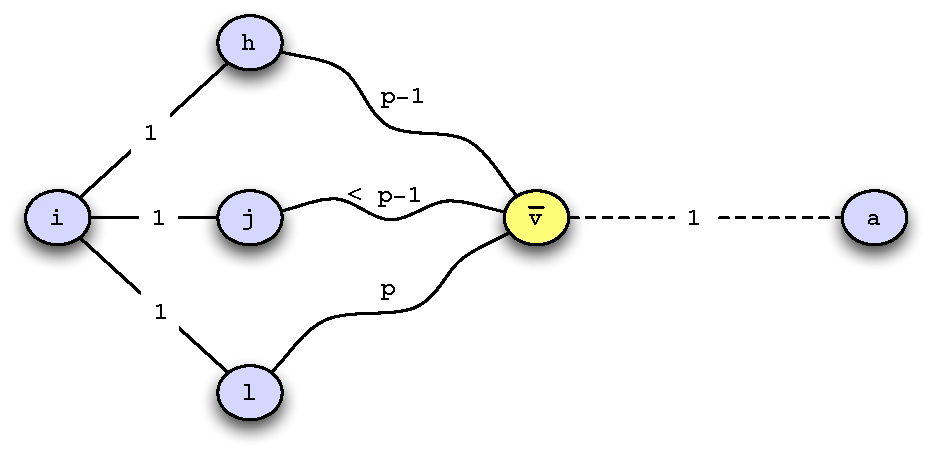
\includegraphics[scale=.57]{figs/second-odd.pdf}
\caption{The yellow node (\bads) is the compromised node.  The dotted line from \bad to $a$ represents the false path. }
\label{fig:second-odd}
\end{figure}

%Intuitively, Theorem \ref{thm:second-odd} establishes that for each destination, $a$, node $i$ counts up by $2$ until reaching value $c$. 
%Node $i$ does so by using allowable paths of length $p^* + 2k$ -- 
%for integers $k \geq 0$ and where $p^*$ is the minimum length path from $i$ to \bad -- and then by uses \bads's false path to destination $a$. 
%These $p^* + 2k$ length paths are derived by hopping back and forth between node $i$ and an adjacent node $j$ 
%(where $j \neq$ \bads) $k$ times and then finally using the path of length $p^*$ from $i$ to \bads.  
%After counting up to $c$ (e.g., when $i$'s least cost to $a$ is $c$), in the next epoch, $i$ uses its path of length
%$p$ to \bads. In the following epoch, $i$ uses its path of length $p+1$ to \bads.  
%From this point, $i$ uses allowable paths of lengths $p+2k$ and $(p+1)+2k$ to \bads, until counting up to $\delta_f(i,j)$.
%For this reason, once $\delta_t(i,j) = c$, $i$ counts up by $1$.



\subsubsection{\cpr Analysis}
\label{subsubsec:cpr-analysis}

The analysis for \second applies to \cpr because after rolling back \cprs, executes the steps of \seconds.  In fact, because \cpr performs the rollback 
using the same diffusing computations analyzed for \second (e.g., the diffusing
computations that remove \bad as a destination), the results for \second apply to \cpr with no changes. %analysis is required for \cprs.  

Although Theorem \ref{thm:second-lbub}, Theorem \ref{thm:second-even}, and Theorem \ref{thm:second-odd} apply directly to \cprs, the bounds and exact message count can defer 
between \second and \cprs. 
%We have already proved in our Technical Report \cite{Tech}, for \cprs, that all nodes correctly rollback to a checkpoint taken before \bad is compromised.  
%Let $\hat{t}$ mark the time \cprs's diffusing computations (to rollback) complete. 
%Because \cpr runs \second at $\hat{t}$, we redefine $C(i,j)$ for \cpr as $C(i,j) = \delta_f(i,j) - \delta_{\hat{t}}(i,j)$.	 
In most cases,  $\delta_{\hat{t}}(i,j)$ for \second is smaller than $\delta_{\hat{t}}(i,j)$ for \cpr because \cpr rolls back to a checkpoint taken before \bad is compromised. 
{\footnote {\small At worst, $\delta_{\hat{t}}(i,j)$ is equivalent across \second and \cprs.  This occurs when the false least vector claimed by \bad matches the least cost
vector used by \bad before being compromised (e.g., \badvectors$=$\oldvectors). }}
Thus, \cprs's $C(i,j)$ values are typically smaller than those for \seconds, resulting in lower message complexity for \cprs.

\subsubsection{\purge Analysis}
\label{subsubsec:purge-analysis}

Our \purge analysis establishes that after the diffusing computations complete, all nodes using false routing state to reach a destination
have a least cost of $\infty$ to this destination.  %Then, control moves back to the neighbors of the compromised node (becausee diffusing computations are initiated from these nodes)
From this point, these least costs remain $\infty$ until updates from nodes with a non-infinite cost to the destination spread through the network.  Upon receiving a non-infinite
least cost to the destination, nodes switch from an infinite least cost to a finite one (Lemma \ref{lem:purge-shrink}).  We establish that the first finite cost to the destination is in fact the node's final correct
least cost to the destination (Theorem \ref{thm:purge-oneupdate}). In this way, least costs change from $\infty$ to their final correct value.
%These correct least costs spread throughout the network until all nodes receive a correct least cost to the destination. % at which point \purge converges
%The correct least costs spread throughout the network and \purge converges on correct least costs when all nodes have received a finite least cost.

In the presence of a tie, we assume a node uses the least cost path that avoids \bads. Note that if ties are broken by using the path with \bad as intermediate node, our
proofs still apply, although with a few minor changes. 
Now we are ready to define two sets that are key structures in our \purge proofs.

\begin{define}
Let $B(a,t)$ be the set of nodes that have least cost $\infty$ to destination node $a$ at time $t$. %$\hat{t}$. %of nodes that have least cost $\infty$ at time $\hat{t}$.
\end{define}

\begin{define}
$F(a,t)$ is the set of nodes such that if $b \in F(a,t)$ then the following must be true:
%$F(a)$ is the set of nodes such that if $b \in F(a)$ then the following must be true at $\hat{t}$:
\begin{enumerate}
	\item $b \notin B(a,t)$.

	\item $\exists b': b' \in adj(b) \wedge b' \notin B(a,t)$.
	%\item $\exists v_{i'j'}: v_{i'j'} \in adj(v_{ij}) \wedge v_{i'j'} \notin B(0)$.
	
	\item $\exists b'': b'' \in adj(b) \wedge b'' \in B(a,t)$.
	%\item $\exists v_{i'j'}: v_{i'j'} \in adj(v_{ij}) \wedge v_{i'j'} \in B(0)$.

\end{enumerate}
\end{define}
%$\forall v_{ij} \in F, \exists v_{i'j'}: v_{i'j'} \in adj(v_{ij}) \wedge v_{i'j'} \notin B(0)$. %$ has $v_j \in adj(v_i): v_j \notin B(0)$. 
% $F$ is the set of all nodes, $v_{ij}$ such that $v_{ij} \notin B(0)$ and 

%\lemma{For an arbitrary $b \in F$ and $a \in V'$, $\ell(b,\overline{v}) = \{\ell(b,a) - 1, \ell(b,a) - 2 \}$

Next, in Lemma \ref{lem:purge-shrink} we prove that the size of $B(a,t)$ shrinks by at least one for each timestep beginning with $t''$ -- where
$t''$ refers to the time that the first $i \in V'$ with $\delta(i,a) = \infty$ changes $\delta(i,a)$ to a finite value -- until $B(a,t)$ is empty.
%This continues until $B(a,t)$ is empty.

\begin{lemma}
\label{lem:purge-shrink}
For each $t \geq t''$, $|B(a,t)| \geq |B(a,t+1)| + 1$, until $B(a,t) = \emptyset$.
%in each subsequent timestep until $B(a) = \emptyset$ at least one node, $j$, changes $\delta(j,a)$ from $\infty$ to a finite value after $\hat{t}$.
\end{lemma}
\begin{proof}
Once \purge diffusing computations complete at $\hat{t}$, a DV computation is triggered at each $v \in adj(\overline{v})$. 
At this point, all least costs corresponding to paths using \bad as an intermediate node are set to $\infty$ (this is proved in Corollary \ref{cor:purge-correct-single}).
As such, each $i \in B(a,\hat{t})$ sends a DV message
with a least of $\infty$ to each neighbor, {\footnote {\small Recall that after $\hat{t}$, \purge forces each node to send a least cost message to each neighbor 
(even if the node's least cost has not changed since $\hat{t}$). }} 
unless $i$ has a neighbor node in $F(a,\hat{t})$ (note that we denote this time as $t''$). 
In this case, $i$ selects a finite least to $a$ (which implies $i \notin B(a,t'')$), triggering the propagation of finite least costs to $a$.  Specifically, in each 
subsequent timestep $t$ (until $B(a,t) = \emptyset$) at least one node, $j$, changes $\delta_t(j,a)$ from $\infty$ to a finite value.  This is the case because unless $B(a,t) = \emptyset$, 
a node $i$ that has changed $\delta_t(i,a)$ from $\infty$ to a finite value, has $j \in adj(i)$ with $\delta_{t}(j,a) = \infty$ and thus $\delta_{t+1}(j,a)$ will be finite.  
A finite $\delta_{t+1}(j,a)$ value implies $j \notin B(a,t+1)$. Since $B(a,t)$ is monotonic, eventually $B(a,t) = \emptyset$. 
%subsequent timestep, $t: t < t^*$, at least one node, $j$, changes $\delta(j,a)$ from $\infty$ to a finite value.  This is the case because at $t-1$, a node $i$ that has changed 
\end{proof}

Our next Lemma (\ref{lem:purge-pathlen}) lists all possible values for the number of links between any $b \in F(a,\hat{t})$ and \bads.  We later use this Lemma in
Theorem \ref{thm:purge-oneupdate}.

\begin{lemma}
\label{lem:purge-pathlen}
For all $b \in F(a,\hat{t})$, $\ell(b,\overline{v}) = \{\ell(b,a), \ell(b,a) - 1\}$.
\end{lemma}
\begin{proof}
Let $b$ be an arbitrary node in $F(a,\hat{t})$.
If $\ell(b,\overline{v}) < \ell(b,a) -1$, this would imply $b \in B(a,\hat{t})$, a contradiction (a violation of condition $1$ of the $F(a,\hat{t})$ definition).  
On the other hand, consider the case where $\ell(b,\overline{v}) > \ell(b,a)$ and where $b' \in adj(b)$ and $b' \in B(a,\hat{t})$.  
Any path $b'$ uses with \bad as an intermediate node has cost
%If $\ell(b,\overline{v}) > \ell(b,a)$ then at $\hat{t}$, $b'$ can use $b$ as a next-hop router with $\delta_{\hat{t}}(b',a)=  \ell(b,a) +1$.  
%While any path $b'$ uses with \bad as an intermediate node has cost
$\ell(b,\overline{v}) -1 + \delta_s(\overline{v},a)  = \ell(b,\overline{v}) -1 + 1 =  \ell(b,\overline{v})$.  Since we have assumed $\ell(b,\overline{v})> \ell(b,a)$,
$b'$ would use $b$ as a next-hop router along $p_{\hat{t}}(b',a)$. 
%{\footnote {\small Note that if $b'$ routes via another node, $b''$, such that $b'' \neq b \wedge b'' \in F(a,\hat{t})$, this would imply $b'' \notin B(a,\hat{t}$. }}
This implies $b'\notin B(a,\hat{t})$, a contradiction. 
\end{proof}

The following theorem is the key argument in establishing \purges's communication complexity.  Theorem \ref{thm:purge-oneupdate} proves that once any $i \in V'$ changes its least cost 
from $\infty$, $i$ changes its least cost to the final correct value.

\begin{theorem}
\label{thm:purge-oneupdate}
For $t > \hat{t}$ and an arbitrary destination $a \in V'$, each $i \in B(a,\hat{t})$ with $\delta_{\hat{t}}(i,a) = \infty$ only modifies $\delta(i,a)$ once,
such that $\delta(i,a)$ changes from $\infty$ to $\delta_f(i,a)$.
\end{theorem}
\begin{proof}
Consider an arbitrary $i \in V'$ such that $i \in B(a,\hat{t})$. $i$ must use some $b \in F(a,\hat{t})$ as an intermediate node along $p_f(i,a)$. % where $a$ is an arbitrary destination.
Let $b^*$ be this node. % (e.g., $b^* \in F(a)$ such that $b^*$ used along $p_f(i,a)$). 
If we show that $\delta_f(b^*,a)$ is the first least cost among all $b \in F(a,\hat{t})$ to reach $i$,
then we have proved our claim because in Lemma \ref{lem:purge-shrink} we proved that $i$ does not update its least cost to a finite value until it receives a least cost from a $b \in F(a,\hat{t})$.
{\footnote {\small  Note that any node $i$ with $\delta(i,a) = \infty$ only changes $\delta(i,a)$ to a finite value. Thus, when \purge forces 
nodes to send a message after $\hat{t}$ to initiate the DV computation, no $i \in B(a,\hat{t})$ receiving a least cost of $\infty$ updates its least cost.}}
For the sake of contradiction, assume that for some $b' \in F(a,\hat{t})$, where $b' \neq b^*$, that $\delta_f(b',a)$ reaches $i$ before $\delta_f(b^*,a)$. 
{\footnote {\small From Lemma \ref{lem:purge-shrink} we know that a finite least cost to $a$ reaches every node in $B(a,\hat{t})$.}}
%{\footnote {\small It is easy to show by induction for an arbitrary $b \in F(a,\hat{t})$ that once a $b' \in adj(b)$,
%modifies for $\delta_t(b',a)$ from $\infty$ to a non-infinite value, that each subsequent timestep, $t < t^*$, at least one node changes its least cost from $\infty$ to a non-infinite value. }}
This implies that:
\begin{eqnarray}
\label{eqn:fcont}
\ell(b',\overline{v}) + \ell(i,b')  &<& \ell(b^*,\overline{v}) + \ell(i,b^*) 
\end{eqnarray}

From Lemma \ref{lem:purge-pathlen}, we know that $\ell(b',\overline{v}) = \{\ell(b',a), \ell(b',a) - 1\}$ and  $\ell(b^*,\overline{v}) = \{\ell(b^*,a), \ell(b^*,a) - 1\}$ 
%It must be the case that $\ell(b',\overline{v}) + 1 = \ell(b',d)$ and $\ell(b^*,\overline{v}) + 1= \ell(b^*,d)$. 
%The other possibility is that $\ell(b',\overline{v}) + 1 = \ell(b',d)$ and $\ell(b^*,\overline{v}) +1 = \ell(b^*,d)$.  
If we substitute  $\ell(b',\overline{v}) = \ell(b',a)$ and $\ell(b^*,\overline{v}) = \ell(b^*,a)$ into Equation \ref{eqn:fcont}, it yields:
\begin{eqnarray}
\label{eqn:purge-contr1}
\ell(b',a) + \ell(i,b')  &<& \ell(b^*,a) + \ell(i,b^*) 
%\ell(i,b') + \ell(b',a) &<& \ell(i,b^*) + \ell(b^*,a) 
\end{eqnarray}
However, since we have assumed that $i$ routes via $b^*$, we know that: 
%This is a contradiction because, we have assumed that $i$ routes via $b^*$, which implies:
\begin{eqnarray}
\label{eqn:purge-contr2}
  \ell(b',a) + \ell(i,b')  &>& \ell(b^*,a) +  \ell(i,b^*) 
  %\ell(i,b') + \ell(b',a) &>&  \ell(i,b^*) + \ell(b^*,a) 
 \end{eqnarray}
Thus, between Equation \ref{eqn:purge-contr1} and Equation \ref{eqn:purge-contr2} we have a contradiction.
Similar contradictions can be derived by substituting all other permutations of the $\ell(b',\overline{v})$ and $\ell(b^*,\overline{v})$ equalities, derived from Lemma \ref{lem:purge-pathlen}.
In conclusion, we have shown by contradiction that $\delta(i,a)$ only changes a single time: $\delta(i,a)$ changes from $\infty$ to $\delta_f(i,a)$.
\end{proof}


\begin{corollary}
\label{cor:purge-loopfree}
\purge is loop-free at every instant of time.
\end{corollary}

\begin{proof}
Before $\hat{t}$, only diffusing computation run. Diffusing computations are loop-free because computation proceeds along spanning trees, which are by definition acyclic. 
After $\hat{t}$, only DV computations run. From Theorem \ref{thm:purge-oneupdate} we know that each node with least cost $\infty$ to an arbitrary destination, changes its least cost once:
from $\infty$ to the correct final least cost. We conclude that \purge is loop free.
\end{proof}

%\begin{proof}
%After the diffusing computations complete, all $\delta(i,j)$ values are either correct or $\infty$.  Jaffe and Moss \cite{JaffMoss} prove 
%DV is loop-free for these exact start conditions.  Since \purge runs
%DV after the diffusing computations complete, we conclude that \purge is loop-free.
%\end{proof}

\begin{theorem}
\label{thm:purge-msg-complexity}
\purge message complexity is $O(mnd)$.
\end{theorem}
\begin{proof}
\purge consists of two steps: the diffusing computations to invalidate false state and DV to compute new least cost paths invalidated by the diffusing computations.
From Lemma \ref{lem:diffuse-total}, \purges's diffusing computations have $O(mE)$ communication complexity.  The DV message complexity can be understood as follows.
To start the computation, \purge enforces that each node sends DV message (to each neighbor), even if no least costs are found. 
From Theorem \ref{thm:purge-oneupdate} and Lemma \ref{lem:purge-shrink}, all $i \in B(a,\hat{t})$ only change $\delta(i,a)$ once: $\delta(i,a)$ changes
from $\infty$ to $\delta_f(i,a)$.  %Therefore, only $O(d)$ timesteps after $t''$ are necessary for all nodes to compute correct least costs to $a$.
\purge computations to all destinations run in parallel, meaning that all least cost updates to nodes $h$ away are handled in the same round of update messages. For this reason,
\purge only sends messages $d+1$ times after $\hat{t}$.  Finally,
since there are $n-1$ nodes, each with a maximum of $m$ neighbors, and each node sends messages $d+1$ times, \purge communication complexity if $O(mnd)$.
%The message complexity if thus for each destination, \purge requires $2d = O(d)$ timesteps after $\hat{t}$ for correct
%least costs to reach all $v \in V'$. Since \purge computations to all destinations run in parallel, only $2d$ timesteps are required for correct least costs to \emph{all} 
%destinations to reach all nodes. 
%Therefore, each node sends a DV message with at least one least cost of $\infty$ at most $2d$ times.  Since there are $n-1$ nodes with a maximum of $n-2$ neighbors, the message complexity 
%contributed by nodes sending least costs of $\infty$ is $O(n^2d)$.
%From Lemma \ref{lem:purge-shrink} and Theorem \ref{thm:purge-oneupdate}, we know that for each destination, \purge requires $2d = O(d)$ timesteps after $\hat{t}$ for correct
%least costs to reach all $v \in V'$. Since \purge computations to all destinations run in parallel, only $2d$ timesteps are required for correct least costs to \emph{all} 
%destinations to reach all nodes. 
%Therefore, each node sends a DV message with at least one least cost of $\infty$ at most $2d$ times.  Since there are $n-1$ nodes with a maximum of $n-2$ neighbors, the message complexity 
%contributed by nodes sending least costs of $\infty$ is $O(n^2d)$.
\end{proof}



\subsubsection{Analysis with Link Cost Changes}
\label{subsubsec:linkchange-complex}


In this section, we analyze each of our algorithms in the case where $w$ link cost changes occur.  Because we assume unit link costs of $1$, a link cost decrease corresponds to the 
addition of a new link and a link cost increase corresponds to the removal of a link.  In our analysis, we assume that all $w$ link cost changes finish propagating before \bad is detected 
(e.g., before $t_b$).

The analysis for \second and \purge from Section \ref{subsubsec:second-analysis} and Section \ref{subsubsec:purge-analysis}, respectively, does not change.  This is the 
case because \second and \purge do not roll back in time, and thus all $w$ link cost changes are accounted for when recovery begins at $t_b$.  
The \cpr analysis from Section \ref{subsubsec:cpr-analysis} changes because after rolling back, all $w$ link cost changes need to be replayed. 

Let $\delta_{f}'(i,a)$ be node $i$'s final least cost to $a$ if no link cost changes occur during $[t',t_b]$.  Define 
$C'(i,j) = \delta_{f}'(i,a) - \delta_{\hat{t}}(i,j)$.

The communication complexity for a link cost increase is $O(n^2)$ \cite{Johnson84} and $O(E)$ for a link cost decrease \cite{Johnson84b}.  Let there be $u$ link cost increases (e.g., $u$ links are 
removed from $G$) and $w-u$ link cost decreases (e.g., $w-u$ links are added to $G$).
At worst, the link cost changes are processed after \bad recovery completes. As a result, \cpr communication complexity with link cost changes is bounded above by:
%with $w$ link cost changes, we now add an $O(wn^2)$ term to Equation \ref{thm:second-ub}:
%The communication complexity for a link cost increase is $O(n^2)$ \cite{Johnson84} and $O(E)$ for a link cost decrease \cite{Johnson84b}.  Thus, link cost increases dominate
%communication complexity. At worst, the link cost changes are processed after \bad recovery completes. As a result, with $w$ link cost changes, we now add an $O(wn^2)$ term to Equation \ref{thm:second-ub}:
\begin{eqnarray}
\label{thm:cpr-link-change}
\sum_{i \in V'} \max_{j \in V', i \neq j} \left( C'(i,j) \right) adj(i) + O(un^2) + O\left((w-u)E\right)
%\sum_{i \in V'} \max \left( \sum_{j \in V', i \neq j} C(i,j) \right) adj(i)
\end{eqnarray}


\subsubsection{Discussion}

The communication complexity for \seconds, \cprs, and \purge are all $O(mnd)$ over graphs with fixed unit link costs.  It is not surprising that the communication complexity is the same 
because all three algorithms use DV as their final step and DV asymptotically dominates the communication complexity of each recovery algorithm. 
In this context, the different performance of our three algorithms --   we find in our simulations --
is determined by the hidden constants. % in the communication complexity results. 

We also bounded the communication overhead of each algorithm under conditions of link cost changes.  \cpr incurred overhead not experienced by \second and \purge because these
two algorithms do not roll back in time and thus all link cost changes are accounted for when recovery begins. % at $t_b$. 




